% \NeedsTeXFormat{LaTeX2e}
\documentclass[12pt,letterpaper]{article}
\renewcommand{\contentsname}{\'Indice}
\usepackage[spanish]{babel}
\usepackage[ansinew]{inputenc}
\usepackage[right=2cm,left=3cm,top=2cm,bottom=2cm,headsep=0cm,footskip=0.5cm]{geometry}
\usepackage[spanish]{isodate}
\usepackage{graphicx}
\usepackage[nobib]{CoverPage}
\usepackage{invoice}
\usepackage{xcolor}
\usepackage{pifont}
\usepackage[dvipdfm hidelinks]{hyperref}
%  usage :example
% \textcolor{Cyan}{\underline{\url{http://www.latex-project.org/}}} 
% \href{http://www.latex-project.org/}{\textcolor{Cyan}{\underline{latex project}}}
% working and tested examples
% 	  \href{run:file.xlsx}{excel}
% 	  \color{kblue}{\url{http://www.latex-project.org/}} 
% 	  \href{http://www.latex-project.org/}{\color{oblue}{{latex project}}}

\hypersetup{colorlinks,backref,%
pdftitle=GST,pdfauthor=GST Departamento de Sistemas,pdfsubject=Quantum Chaos,%
pdfpagemode=FullScreen}


\usepackage{pgf,tikz}
\usetikzlibrary{shapes,arrows,calc,positioning}

%%%%%%%%%%%%%%%%%%%%%%%%%%%%%%%%%%%%%%%%%%%
\usepackage{fancyhdr}  %% Make headers

\pagestyle{fancy}
% \fancyhf{}
% \rhead{Reunion Preliminar}
% \lhead{Manual de Procedimientos}
% \rfoot{
% 	\vfill{\hrule
% 	\vspace{5mm}
% 	}
% % 	\textsuperscript{*} Example ...
% %   P\'agina \thepage
%   }
% \renewcommand{\headrulewidth}{0.4pt}
\renewcommand{\footrulewidth}{0.4pt}
\fancyfoot[C]{\bfseries \thepage} % except the center
\rfoot{\today}
\headsep 15pt
\footskip 10pt
%%%%%%%%%%%%%%%%%%%%%%%%%%%%%%%%%%%%%%%%%%
\definecolor{kblue}{HTML}{29576B}
\definecolor{kgreen}{HTML}{1A3931}
\definecolor{oblue}{HTML}{09D4FF}
\definecolor{kgray}{HTML}{3A3A3A}
\definecolor{alert}{HTML}{C21B4D}
\definecolor{lavander}{cmyk}{0,0.48,0,0}
\definecolor{violet}{cmyk}{0.79,0.88,0,0}
\definecolor{burntorange}{cmyk}{0,0.52,1,0}
%             \def\tableofcontents{\@restonecolfalse
%               \if@twocolumn\@restonecoltrue\onecolumn\fi
%               %\chapter*{\,%\contentsname
%               %     \@mkboth{\uppercase{\contentsname}}{\uppercase{\contentsname}}
%               %    }%
%               %\clearpage
%               \begin{center}
%                     \MakeUppercase{\contentsname}
%               \end{center} \par
% 			  %
% 			  {\ssp\@starttoc{toc}}\if@restonecol\twocolumn\fi}
%%%%%%%%%%%%%%%%%%%%%%%%%%%%%%%%%%%%%%%%%%%%%%%%%%%%%%%%%%%%%%%%%%%%%%%%%%%%%%%%
% maybe works
\makeatletter
\def\thickhrulefill{\leavevmode \leaders \hrule height 1pt\hfill \kern \z@}
\def\makecaratula{%
  \null
  \thispagestyle{empty}%
  
%   \begin{center}
% %     \huge \strut \@title \par
%     \huge \strut \@institute \par
%   \end{center}
  
  \vskip 1cm
  \begin{flushright}
    \scshape\Large\@author
  \end{flushright}
  \vfil
  \hrule height 2pt
  \par
  \begin{center}
%     \huge \strut \@title \par
    \normalfont \strut \@title \par
  \end{center}
  \hrule height 2pt
  \par
  \vfil
  \vfil
  \null
  \cleardoublepage
  }
\makeatother
% \author{Isidore Ducasse, Comte de Lautréamont}
\author{Objetivo del Procedimiento}
\title{Fijar el compromiso entre las partes involucradas para realizar el plan de trabajo del Presupuesto , resolviendo dudas,descubriendo puntos ciegos y homologando procesos.}
% \institute{
% 	Procedimiento Elaboracion de Presupuesto GST 2014.
%   }
% \date{2014}
%%%%%%%%%%%%%%%%%%%%%%%%%%%%%%%%%%%%%%%%%%%%%%%%%%%%%%%%%%%%%%%%%%%%%%%%%%%%%%%%
%-----------------------------------------------------------------------
\CoverPageSetup{title=Manual de Presupuesto GST,author=Manual de Procedimientos del Grupo de Servicios de Transporte para la Reunion Preliminar,institute={Bonampak\texttrademark \\ Gerencia de Aministraci\'on y Finanzas},insource={\emph{guillermo.rodriguez@bonampak.com.mx}},copyright={\copyright{GST Departamento de Sistemas} } }

\renewcommand{\CoverPageHeader}{%
  {
\includegraphics[width=176mm]{img/corporate.png}}%
}
\renewcommand{\CoverPageFooterLogo}{
\includegraphics[width=.15\textwidth]{/media/sdb1/data/books/latex/src/xdosemu.png}}

%-----------------------------------------------------------------------%

\begin{document}

\makecaratula
\newpage

 {\sffamily % Start the Document
  % for smallcaps shape use the command \scshape
  \title{\scshape Procedimiento para realizar la Reuni\'on Preliminar del Grupo de Servicios de Transporte}
  \author{\copyright Bonampak}
  \maketitle

  \tableofcontents
    \listoffigures

  \newpage
%% Begin the maths
  %%% Reunion Preliminar %%%
  \begin{section}
  {\color{kblue} Procedimiento de la Reuni\'on Preliminar GST}
	
	\vspace{17mm}
    \begin{subsection}
    {\color{kgreen}Apertura Oficial }
	  Consiste en la apertura oficial del Presupuesto con una breve introducci\'on por parte de la Direcci\'on General y la entrega de Documentos de expectativas.
	  \\
    \end{subsection}
%       \newpage

 
    \begin{subsection}
% 	\vheight{70mm}
	{\color{kgreen}Fijar Objetivos y Par\'ametros Generales}
	  El Coordinador presenta y fija los objetivos concretos , par\'ametros generales que son la base para realizar el Proyecto de Presupuesto para GST.
    \end{subsection}
    
%       \newpage
%     \vspace{70mm}
    \begin{subsection}
    {\color{kgreen}Presentaci\'on de resultados y \'ultimo estimado}
	  Posteriormente el Coordinador presenta a la Asamblea reunida las expectativas y relevancias para el pr\'oximo a\~no por medio de Presentaciones , diapositivas y material necesario que sirva para una mejor comprensi\'on de los presentes
	  \\
    \end{subsection}
    
    
%       \newpage
%       \vspace{70mm}
    \begin{subsection}
    {\color{kgreen}Compromiso General}
El Coordinador tiene que asegurar el compromiso de la Asamblea compuesta por Gerencia General , Gerencias de Area , Gerencias de Base y Supervision de Bases , logrando llegar a acuerdos en el cumplimiento con el plan de trabajo y los objetivos expuestos anteriormente
	  \\
    \end{subsection}
    
      \newpage
%       \vspace{70mm}
    \begin{subsection}
    {\color{kgreen}Cronograma}
Por \'ultimo el Coordinador presenta el cronograma \ref{crono} en el cual est\'an fijados los tiempos de entrega de cada uno de los procesos para la Elaboracion  del Presupuesto GST.
  \begin{center}
  
		\begin{figure}[htb]
		    \centering
		    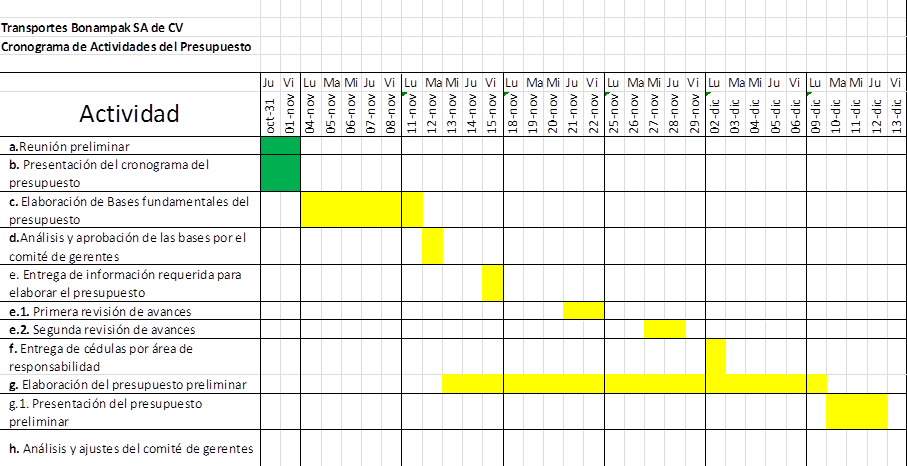
\includegraphics[angle=0,width=150mm]{img/cronograma.png}
		    \caption{Cronograma}
		    \label{crono}
		\end{figure}
	\end{center}
	  \\
    \end{subsection}
    
      \newpage
%       \vspace{70mm}
    \begin{subsection}
    {\color{kgreen}Fin de la Reuni\'on Preliminar}
	  El Coordinador dara por terminada la reunion preliminar informando la fecha para la siguiente Reuni\'on
	  \\
    \end{subsection}
    
%     \newpage
%     \begin{subsection}
% 		{\color{kgray}Diagrama de Flujo}
% %     \end{subsubsection}
%   \begin{center}
%   
% 		\begin{figure}[htb]
% 		    \centering
% 		    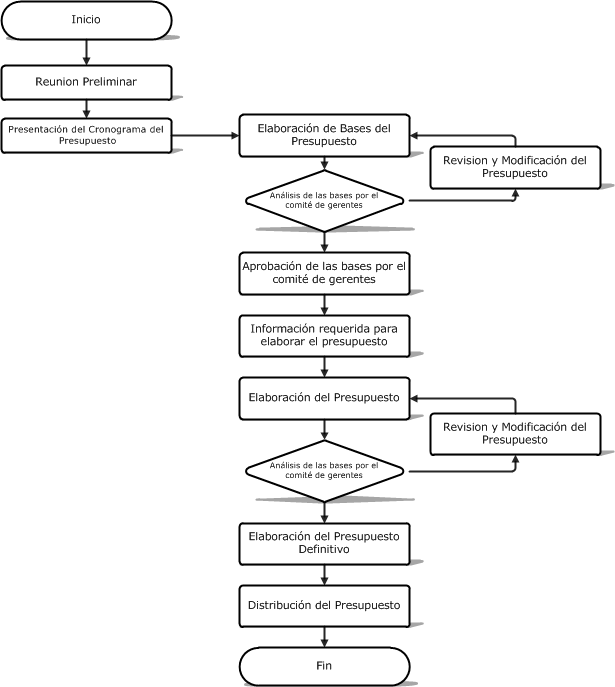
\includegraphics[angle=0,width=150mm]{img/dia/Presupuesto_General_tab_b.png}
% 		    \caption{Elaboraci\'on del Presupuesto GST}
% 		    \label{luna}
% 		\end{figure}
% 	\end{center}
%   \end{subsection}
%  
% 	\newpage
	
% 	\begin{itemize}
% 	\item[\ding{229}]{}
% 
% 	\begin{itemize}
% 	    \item[\ding{237}]{...
% 	%imagenes only 3 figures are allowed per page
% 		\begin{figure}[htb]
% 		    \centering
% 		    \includegraphics[angle=0,width=4mm]{moon.png}
% 		    \caption{caption}
% 		    \label{luna}
% 		\end{figure}
% 	    }
% 	\end{itemize}
% 
% 	\begin{itemize}
% 	    \item[\ding{237}]{...
% 		\begin{figure}[htb]
% 		    \centering
% 		    \includegraphics[angle=0,width=4mm]{moon.png}
% 		    \caption{caption}
% 		    \label{luna}
% 		\end{figure}
% 	    }
% 	\end{itemize}
% 
% 	\begin{figure}[htb]
% 	    \centering
% 	    \includegraphics[angle=0,width=4mm]{moon.png}
% 	    \caption{caption}
% 	    \label{luna}
% 	\end{figure}
% 
% 	
% 	%lista
% 	\begin{itemize}
% 	\item[\ding{182}]{ list \ding{231} \includegraphics[angle=0,width=4mm]{moon.png}}
% 	\end{itemize}
%     \end{itemize}
% %     \vfill{\hrule
% % 	\vspace{5mm}
% % 	\textsuperscript{*} Example ...
% %     }
%   \end{section}
% 
% 
%   \newpage
%   \begin{section}
%   {\color{kblue} Cronograma}
% 
%     \begin{subsection}
%     {\color{kgreen}subsection ...}
%     \end{subsection}
% 
%     \begin{subsubsection}
%     {\color{kgray}Sub---subsection ...}
%     \end{subsubsection}
% 
%     \begin{itemize}
% 	\item[\ding{229}]{...}
% 
% 	\begin{itemize}
% 	    \item[\ding{237}]{...
% 	%imagenes only 3 figures are allowed per page
% 		\begin{figure}[htb]
% 		    \centering
% 		    \includegraphics[angle=0,width=4mm]{moon.png}
% 		    \caption{caption}
% 		    \label{luna}
% 		\end{figure}
% 	    }
% 	\end{itemize}
% 
% 	\begin{itemize}
% 	    \item[\ding{237}]{...
% 		\begin{figure}[htb]
% 		    \centering
% 		    \includegraphics[angle=0,width=4mm]{moon.png}
% 		    \caption{caption}
% 		    \label{luna}
% 		\end{figure}
% 	    }
% 	\end{itemize}
% 
% 	\begin{figure}[htb]
% 	    \centering
% 	    \includegraphics[angle=0,width=4mm]{moon.png}
% 	    \caption{caption}
% 	    \label{luna}
% 	\end{figure}
% 	
% 	\footnotesize{\scshape{
% 	  \begin{invoice}{MXN}{0}
% 	    \ProjectTitle{\color{red}Costos por Unidad de Negocio}%
% 	    
% 	    \Fees{s  Por 4 Modulos}{ .... }{}
% 	    \Fee{...}{2000}{1}
% 	    \Fee{...}{2000}{1}
% % 	    \Fee{Control Unidades Fuera de la Ciudad}{2000}{1}
% % 	    \Fee{Control de Unidades en Servicio}{2000}{1}
% % 	    \Fee{Servidor 1 a\~no 24-hrs/365-dias}{2000}{1}
% % 	    \Discount{1 Modulo Gratis}{2000}
% 	  \end{invoice}
% 	    }%end of size
% 	  }%end of smallcaps
% 	  
% 	%lista
% 	\begin{itemize}
% 	\item[\ding{182}]{ list \ding{231} \includegraphics[angle=0,width=4mm]{moon.png}}
% 	\end{itemize}
%     \end{itemize}
% %     \vfill{\hrule
% % 	\vspace{5mm}
% % 	\textsuperscript{*} Example ...
% %     }
%   \end{section}
% 
% \newpage
% 
%   \begin{section}
%   {\color{kblue} Bases Fundamentales}
% 
%     \begin{subsection}
%     {\color{kgreen}Recopilar informacion de las Unidades de Negocio}
%     \end{subsection}
% 
%     \begin{subsubsection}
%     {\color{kgray}Delegar Responsabilidades ...}
%     \end{subsubsection}
% 
%     \begin{itemize}
% 	\item[\ding{229}]{...}
% 
% 	\begin{itemize}
% 	    \item[\ding{237}]{...
% 	%imagenes only 3 figures are allowed per page
% 		\begin{figure}[htb]
% 		    \centering
% 		    \includegraphics[angle=0,width=4mm]{moon.png}
% 		    \caption{caption}
% 		    \label{luna}
% 		\end{figure}
% 	    }
% 	\end{itemize}
% 
% 	\begin{itemize}
% 	    \item[\ding{237}]{...
% 		\begin{figure}[htb]
% 		    \centering
% 		    \includegraphics[angle=0,width=4mm]{moon.png}
% 		    \caption{caption}
% 		    \label{luna}
% 		\end{figure}
% 	    }
% 	\end{itemize}
% 
% 	\begin{figure}[htb]
% 	    \centering
% 	    \includegraphics[angle=0,width=4mm]{moon.png}
% 	    \caption{caption}
% 	    \label{luna}
% 	\end{figure}
% 	
% 	\footnotesize{\scshape{
% 	  \begin{invoice}{MXN}{0}
% 	    \ProjectTitle{\color{red}Costos por Unidad de Negocio}%
% 	    
% 	    \Fees{s  Por 4 Modulos}{ .... }{}
% 	    \Fee{...}{2000}{1}
% 	    \Fee{...}{2000}{1}
% % 	    \Fee{Control Unidades Fuera de la Ciudad}{2000}{1}
% % 	    \Fee{Control de Unidades en Servicio}{2000}{1}
% % 	    \Fee{Servidor 1 a\~no 24-hrs/365-dias}{2000}{1}
% % 	    \Discount{1 Modulo Gratis}{2000}
% 	  \end{invoice}
% 	    }%end of size
% 	  }%end of smallcaps
% 	  
% 	%lista
% 	\begin{itemize}
% 	\item[\ding{182}]{ list \ding{231} \includegraphics[angle=0,width=4mm]{moon.png}}
% 	\end{itemize}
%     \end{itemize}
% %     \vfill{\hrule
% % 	\vspace{5mm}
% % 	\textsuperscript{*} Example ...
% %     }
%   \end{section}
% %%%%%%%%%%%%%%%%%%%%%%%%%%%%%%%%%%%%%%%%%%%%%%%%%%%%%
% 
% 
%   %%% Squeleton %%%
% %   \begin{section}
% %   {\color{kblue} Section...}
% % 
% %     \begin{subsection}
% %     {\color{kgreen}subsection ...}
% %     \end{subsection}
% % 
% %     \begin{subsubsection}
% %     {\color{kgray}Sub---subsection ...}
% %     \end{subsubsection}
% % 
% %     \begin{itemize}
% % 	\item[\ding{229}]{...}
% % 
% % 	\begin{itemize}
% % 	    \item[\ding{237}]{...
% % 	%imagenes only 3 figures are allowed per page
% % 		\begin{figure}[htb]
% % 		    \centering
% % 		    \includegraphics[angle=0,width=4mm]{moon.png}
% % 		    \caption{caption}
% % 		    \label{luna}
% % 		\end{figure}
% % 	    }
% % 	\end{itemize}
% % 
% % 	\begin{itemize}
% % 	    \item[\ding{237}]{...
% % 		\begin{figure}[htb]
% % 		    \centering
% % 		    \includegraphics[angle=0,width=4mm]{moon.png}
% % 		    \caption{caption}
% % 		    \label{luna}
% % 		\end{figure}
% % 	    }
% % 	\end{itemize}
% % 
% % 	\begin{figure}[htb]
% % 	    \centering
% % 	    \includegraphics[angle=0,width=4mm]{moon.png}
% % 	    \caption{caption}
% % 	    \label{luna}
% % 	\end{figure}
% % 	
% % 	\footnotesize{\scshape{
% % 	  \begin{invoice}{MXN}{0}
% % 	    \ProjectTitle{\color{red}Costos para la Unidad de Negocio}%
% % 	    
% % 	    \Fees{s  Por 4 Modulos}{ .... }{}
% % 	    \Fee{...}{2000}{1}
% % 	    \Fee{...}{2000}{1}
% % % 	    \Fee{Control Unidades Fuera de la Ciudad}{2000}{1}
% % % 	    \Fee{Control de Unidades en Servicio}{2000}{1}
% % % 	    \Fee{Servidor 1 a\~no 24-hrs/365-dias}{2000}{1}
% % % 	    \Discount{1 Modulo Gratis}{2000}
% % 	  \end{invoice}
% % 	    }%end of size
% % 	  }%end of smallcaps
% % 	  
% % 	%lista
% % 	\begin{itemize}
% % 	\item[\ding{182}]{ list \ding{231} \includegraphics[angle=0,width=4mm]{moon.png}}
% % 	\end{itemize}
% %     \end{itemize}
% %     \vfill{\hrule
% % 	\vspace{5mm}
% % 	\textsuperscript{*} Example ...
% %     }
% %   \end{section}

 }% end of serif font family

\end{document}
